%\documentclass[a4paper,10pt]{article}
%\usepackage[utf8]{inputenc}
%\usepackage{graphicx}
%\usepackage{url}

%opening
%\title{Evacuation Simulator}
%\author{Team L}

%\begin{document}

%\maketitle

%\begin{abstract}
%It is acknowledged that the cost of 
%running evacuation drills in pubilc environments is relatively high both in time and money. This is because very often, the 
%evacuation drills have to be run at night where the chosen environment is not in service and consequently additional payments for 
%equipments, hiring evacuees and fire consultant are needed. This results in fewer number of evacuation drills. 
%There are also some types of evacuation that cannot be drilled both safely and accurately such as a large fire.
%An evacuation simulator is a possible solution to these problems which uses human behaviour in evacuation environment 
%to predict the egress of a population. The aim of this project involves producing a three dimensions visualised 
%evacuation simulator at The Tall Ship at Riverside, Glasgow. Not only focussing on implementation side, the research 
%side is essentially indispensable. Psychology of mass emergency evacuation behaviour and crowd patterns are applied in 
%order to best determine how people will react in an evacuation situation. Moreover, several path finding algorithms 
%are studied to find out which one is suitable for the project.
%The implementation side of this project 
%involves the modelling of the chosen environment in 3D visualisation and simulating an evacuation on this model.
%With this combination, evacuation simulator is more realistic.
%\end{abstract}
%
%\tableofcontents

\section{Introduction}

\subsection{Motivation}
Fatalities and injuries may be due to not only the nature of the disaster or emergency itself - whether a fire, 
bombing, sinking ship, or train or plane crash - but also human factors(behaviour of the evacuating crowd)~\cite[Section 1.1]{psychology}. These human factors include not only 
the effectiveness and appropriateness of emergency procedures and services, but also the behaviour of the evacuating crowd,
which has often been blamed for panic, disorganized, over-emotional, irrational and ineffective egress~\cite[Section 1.2]{psychology}. 
Other human factors which may play a role include decision-making~\cite[Section 2.2]{psychology} and the interpretation of events~\cite[Section 2.3]{psychology}
, leadership and social influence~\cite[Section 2.9]{psychology}, 
and after-care policies and practices~\cite[Section 3: Social Identity]{psychology}.Therefore, building an evaucation simulator which corresponds to the behaviour 
of evacuating crowd might help reduce fatalities and injuries within less time and budget.

\subsection{Definition of an Evacuation Simulator}
An evacuation simulator can be defined as a system to determine evacuation
times by predicting the egress of individuals in a building or similar
structure~\cite{evacuationSimulatordefinition}. They are used to identify
fication of weaknesses in the design of buildings which could detrimentally affect
the egress of persons in an evacuation and to aid personnel in
preparing for an evacuation~\cite{evacuationModel}.

\subsection{Why Implement an Evacuation Simulator}
The task of testing a building's evacuation procedure can be
both difficult and expensive. One approach is to hire members of the public
as stand-in ``evacuees'' and run a mock evaluation, such as those performed as part of Forward Defensive
in preparation for the London 2012 Olympics \cite{DailyMailEvacuation}. In theory this would allow an 
appropriate expert such as a consultant from a local fire department to assess the effectiveness
of an existing plan. However such tests on public buildings can be very expensive: the cost
of hiring evacuees could be significant. Also certain aspects of evacuations, such
as testing the possibility of a crush, can expose participants
to real danger. Finally if an evacuee knows they are participating in an experiment
their behaviour is inherently different than it would be in a real evacuation. This
phenomenon is known as Evaluation Apprehension\cite{EvalApprehension}.\\
For these reasons large scale tests on a building are rarely performed.
What a simulator provides is a means for an expert to extensively test the outcomes of evacuating a location
at minimal cost. By configuring variables in the simulation the expert can examine the probable outcome of multiple evacuations
and look for potential sources of danger in a building or evacuation procedure.

\subsection{Aims}
The Evacuation Simulation project’s aims are building a visual simulator that
can be used on a wide range of structures, for which models can be imported in
the final software without requiring extensive knowledge of the coding process.
Once the software is available to fire wardens or other authorities in charge of
building safety, they can cheaply run computer simulations on buildings and,
depending on the results provided, identify areas where improvements can be
made. Such improvements could be supplementing fire personel and/or fire
extinguishing equipment, opening alternative evacuation routes,
informing the intervening fire brigade of any areas with low evacuation rates etc.
This project intends to simulate an evacuation of The Tall Ship at Riverside(reasons why choosing the environment are explained in section 2),
Glasgow, in a virtual 3D environment. 
Specifically, the evacuation simulator is
expected to be able to accurately model the behaviour of people as they egress
from the ship and provide an interactive graphical user interface which gives
real-time feedback on the current state of all passengers.
It was decided to work towards an evacuation of the ship where the cause is
fire. This will require the exploration of various models of fire~\cite{fireEvacuationProcedure} and the challenge
of integrating it into the final evacuation system. It will also allow us to explore
the impact of smoke on the subjects within the ship.
The aim of this project is to produce a product which gives a
reasonably accurate representation of the egress of people which can hopefully
aid The Tall Ship in planning for an evacuation. The finished product can be
extended to include extra features, such as an enhanced fire model, to make the
simulation more realistic.

\subsubsection{A Multi-Agent Model of Individuals and Individual Behaviour}
Previous projects have emphasised crowd behaviour: they have modelled the population from a top down 
perspective with little consideration for the perception and interaction which an individual experiences in an evacuation.
One of the primary aims of this project is to represent a accurate model of individual behaviour.
Previous work has shown that multi-agent systems can achieve this. By taking this approach "the full effects of diversity that exists among agents in their attributes and behaviours can be observed as it
gives rises to the behaviour of the system as a whole" \cite{AgentBasedTutorial}.

\subsubsection{An Update of the Technologies Used in Previous Projects}
Many previous works in this field have made use of software packages such as Java 3D; these are now unsupported and 
would be difficult to extend in the future.
These are discussed in the Implementation section.

\subsubsection{Use of Navigation Meshes in Environment Modelling}
A Navigation Mesh is a graph representation of an environment in terms of a set of convex polygons which describe the `walkable' surface of an environment. This design aids agents in finding paths through large areas, whilst avoiding static obstacles in the environment.
This technique has largely been pioneered in Gaming, but is equally applicable in this setting. The benefits of a navigation mesh, or 'navmesh' is that it allows agents to move 
freely compared to other techniques such as representing the environment using a grid. A navmesh is typically combined with the powerful path finding algorithm A* to 
optimise agent movement \cite{A*Review}.

\subsection{Prerequisites}
Where possible all technical concepts used within this paper will be clearly defined. However, To fully understand the remainder of this report, the reader should have at least
minimum knowledge in the following areas:
\begin{itemize}
 \item Object-Oriented programming concepts (preferably in Java)
 \item Concurrent programming concepts
 \item Pathfinding simulation and collision detectance/avoidance~\cite{gameProgramming}~\cite{collisionDetection}
 \item Herding, flocking behaviour and boids~\cite{HAndBoid}~\cite{Fbehavior}
 \item Human behavioural traits~\cite{HumanBehaviouralTraits}
 \item 3 Dimentional Vectors
\end{itemize}

\subsection{Previous Work}

\subsubsection{Fluid Based Systems}
These systems model crowd movement as if the crowd were a fluid \cite{WikipediaFluidMechanics}, using equations and principles taken from Physics. 
Exodus \cite{GaleaNumericalSimulation,GaleaMathModelling} is an example of such a system. There are drawbacks in such a style 
of simulator. Crowds "have a choice in their direction, they have no conservation of momentum and can stop and start at will" \cite{StillCrowdDynamics}. 
These concepts are not accounted for in fluid models, and so this style of simulator is limited to estimating the movement of a crowd as a whole without
considering individual interactions.

\subsubsection{Matrix or Grid Based Systems}
In a matrix or grid based system, the floor of the environment is represented by a series of adjacent nodes, often square or hexagonal in shape. Each 
cell can represent open areas, areas blocked by a static obstacle, exits, etc. This method is becoming less common, but two formerly well know examples are 
Egress and Pedroute. It was suggested that the existing matrix-based models suffer from the
difficulties of simulating crowd cross flow and concourses; furthermore, the
assumptions employed in these models are questionable when compared with field observations \cite{StillCrowdDynamics}.

\subsubsection{Emergent Agent Based Systems}
The final class of simulator we discuss here is the emergent (agent based) simulator. In this approach the system is composed of autonomous
and interacting ``agents''. Agents interact within an environment using a defined set of simple relationships. The benefit of this approach is the introduction
of \emph{emergent} behaviour: ``patterns, structures and behaviours emerge that were not explicitly programmed into the models, but arise as the 
result of agent interactions'' \cite{AgentBasedTutorial}.\\
The MASSEgress project developed at Stanford University is an ongoing effort to develop a framework for the development of such systems \cite{MultiAgentFramework}.
It has also led to the production of at least one prototype implementing this framework. 
This project has utilised a modified version of this framework for the integration
of agent behaviour. This is discussed further in the Research and Implementation sections.

\subsection{Background}
At present, previous works discussed in last section are obsolete, as they were designed to use Java3D~\cite{java3D},
an old and currently unsupported library. JMonkeyEngine~cite{jmonkey} was chosen as a
replacement 3D development engine for this project. This is an open source
tool and has an active community surrounding it, which could help with solving
eventual problems that might appear when using it.
While some of the previous projects have flaws that make them unusable for
simulation of large environments~\cite{glasgowUSimulator}, one the current project’s main purposes is
scalability - importing of reasonably large building models and, once imported,
executing simulation on the resulted logical structure in a reasonable time-frame.

\section{Environment}
The Glenlee, the tall ship, was built at the Bay Yard in Port Glasgow and was one of a group of 10 steel sailing vessels 
built to a standard design for the Glasgow shipping firm of Archibald Sterling and Co. Ltd. 
She is a three masted barque, with length 245 feet, beam 37.5 feet and depth 22.5 feet.
The Glenlee first took to the water as a bulk cargo carrier in 1896. She circumnavigated the globe four times
and survived passing through the fearsome storms of Cape Horn 15 times before 
being bought by the Spanish navy in 1922 and being turned into a sail training vessel. 
The ship was modified and served in that role until 1969. She then operated as a training school until 1981 
when she was laid up in Seville Harbour and largely forgotten.
Nowadays, she is permanently docked at the Riverside Museum in Glasgow which operates a programme of year-round maritime 
themed events and activities, with specially devised talks and tours, school visits and costumed volunteer days.

\begin{center}
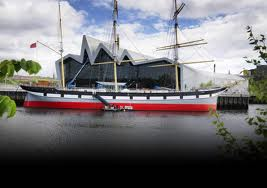
\includegraphics{../images/glasgowTallShip.jpg}
\\Figure 1: Glasgow Tall Shap
\end{center}
Current work on the project is based on evacuating The Tall Ship because 
\begin{itemize}
 \item It serves as both a tourist attraction and a function hall below decks.
 \item The ship is permanently docked and can be considered a static structure.
 \item Events can host up to 200 guests, excluding staff.
 \item It has a sufficiently complex structure in which to explore simulation techniques.
 \item No full scale evacuations have ever been held before - only staff have been used.
 \item These drills are infrequent.
\end{itemize}

\begin{center}
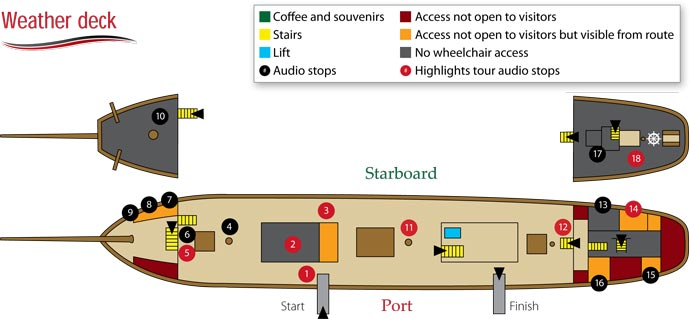
\includegraphics[scale=0.4]{../images/weatherdeck.jpg}
\\Figure 2: Weather Deck
\end{center}

\begin{center}
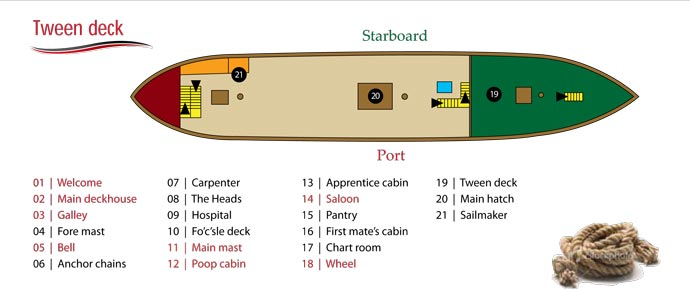
\includegraphics[scale=0.4]{../images/tweendeck.jpg}
\\Figure 3: Tween Deck
\end{center}

\begin{center}
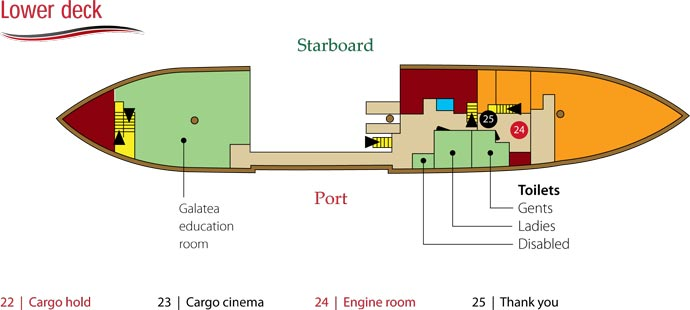
\includegraphics[scale=0.4]{../images/lowerdeck.jpg}
\\Figure 4: Lower Deck
\end{center}

\begin{center}
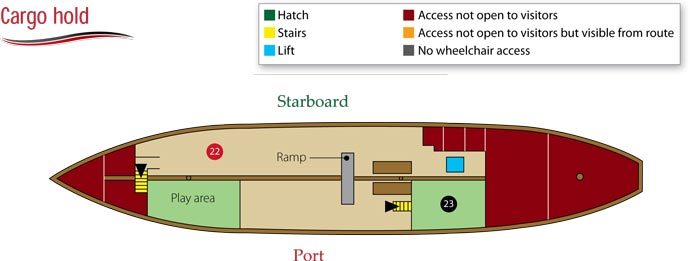
\includegraphics[scale=0.4]{../images/cargohold.jpg}
\\Figure 5: Cargo Hold
\end{center}

It is important to note that only small scale staff evacuations have been conducted on the ship
thus far considering the impractical nature of carrying out an evacuation with
actual visitors. Because of this restriction, an evacuation simulation of The
Tall Ship is ideal to assess the safety of visitors on the ship in the event of an
emergency evacuation.

%\bibliographystyle{unsrt}   % this means that the order of references
%			    % is dtermined by the order in which the
%			    % \cite and \nocite commands appear
%\bibliography{individual_ref}

%\end{document}
